Performance evaluation for each tool-chain is based on time taken for all steps needed to go from source to bit-stream. Each test is run twice to also measure total time on consecutive executions. This was needed as some tool-chains generate IP cores the first time used and that contributes to overall performance time.

IceStudio is using APIO under the hood so performance should be almost identical

Performance times are shown for LED Blinker project (Figure \ref{fig:led_blinker_times}) and SimpleCounter project (Figure \ref{fig:counter_times})
\begin{figure}
    \centering
    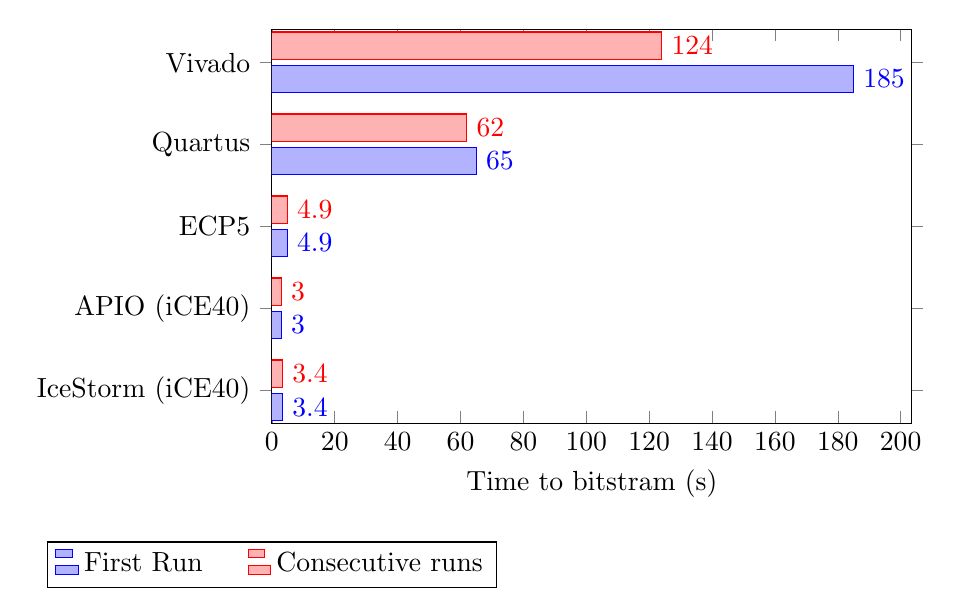
\begin{tikzpicture}
        \begin{axis}[ 
        scale only axis, % The height and width argument only apply to the actual axis
        height=5cm,
        width=\textwidth-4cm,
        xbar, xmin=0,
        xlabel={Time to bitstram (s)},
        symbolic y coords={%
            {IceStorm (iCE40)},
            {APIO (iCE40)},
            {ECP5},
            {Quartus},
            {Vivado}
            },
        ytick=data,
        nodes near coords, 
        nodes near coords align={horizontal},
        ytick=data,
        legend style={
            at={(0,-0.3)},
            anchor=north,
            legend columns=-1,
            /tikz/every even column/.append style={column sep=0.5cm}
        },
        ]
        \addplot coordinates {
            (3.4,{IceStorm (iCE40)}) 
            (3.0,{APIO (iCE40)})
            (4.9,{ECP5}) 
            (65,{Quartus}) 
            (185,{Vivado})};
        \addplot coordinates {
            (3.4,{IceStorm (iCE40)}) 
            (3.0,{APIO (iCE40)})
            (4.9,{ECP5}) 
            (62,{Quartus}) 
            (124,{Vivado})};
        \legend{First Run, Consecutive runs}
        \end{axis}
    \end{tikzpicture}
    \caption{LED Blinker time}
    \label{fig:led_blinker_times}
\end{figure}

\begin{figure}
    \centering
    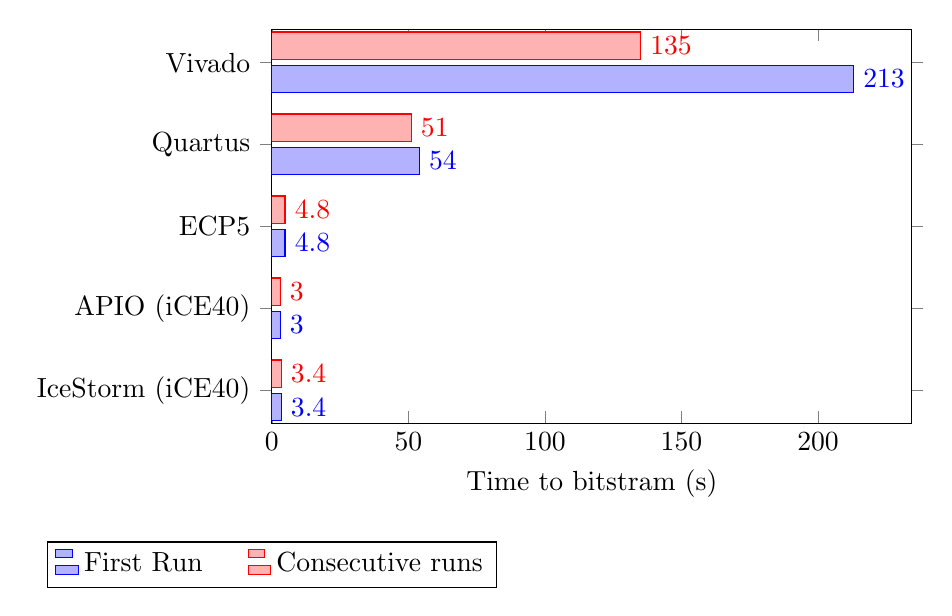
\begin{tikzpicture}
        \begin{axis}[ 
        scale only axis, % The height and width argument only apply to the actual axis
        height=5cm,
        width=\textwidth-4cm,
        xbar, xmin=0,
        xlabel={Time to bitstram (s)},
        symbolic y coords={%
            {IceStorm (iCE40)},
            {APIO (iCE40)},
            {ECP5},
            {Quartus},
            {Vivado}
            },
        ytick=data,
        nodes near coords, 
        nodes near coords align={horizontal},
        ytick=data,
        legend style={
            at={(0,-0.3)},
            anchor=north,
            legend columns=-1,
            /tikz/every even column/.append style={column sep=0.5cm}
        },
        ]
        \addplot coordinates {
            (3.4,{IceStorm (iCE40)}) 
            (3.0,{APIO (iCE40)})
            (4.8,{ECP5}) 
            (54,{Quartus}) 
            (213,{Vivado})};
        \addplot coordinates {
            (3.4,{IceStorm (iCE40)}) 
            (3.0,{APIO (iCE40)})
            (4.8,{ECP5}) 
            (51,{Quartus}) 
            (135,{Vivado})};
        \legend{First Run, Consecutive runs}
        \end{axis}
    \end{tikzpicture}
    \caption{Counter time}
    \label{fig:counter_times}
\end{figure}

